\paragraph{QuizziPedia::Front-End::ModelViews::QuestionsManagementModelView}

\label{QuizziPedia::Front-End::ModelViews::QuestionsManagementModelView}

\begin{figure}[ht]
	\centering
	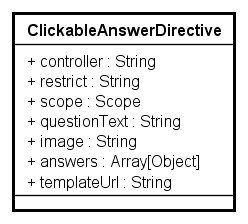
\includegraphics[scale=0.5,keepaspectratio]{UML/Classi/Front-End/QuizziPedia_Front-end_Templates_ClickableAnswerTemplate.png}
	\caption{QuizziPedia::Front-End::ModelViews::QuestionsManagementModelView}
\end{figure} \FloatBarrier

\begin{itemize}
	\item \textbf{Descrizione}: classe di tipo modelview la cui istanziazione è contenuta all'interno della variabile di ambiente \$scope di \textit{Angular.js\ped{G}}. All'interno di essa sono presenti le variabili e i metodi necessari per il \textit{Two-Way Data-Binding\ped{G}} tra la view \texttt{QuestionsManagementView} e il controller \texttt{QuestionsManagementController};
	\item \textbf{Utilizzo}: viene utilizzata per effettuare il \textit{Two-Way Data-Binding\ped{G}} tra la view \texttt{QuestionsManagementView} e il controller \texttt{QuestionsManagementController} rendendo disponibili variabili e metodi;
	\item \textbf{Relazioni con altre classi}: 
	\begin{itemize}
		\item \textit{IN} \texttt{QuestionsManagementView}: view contenente l’elenco delle domande create; 
		\item \textit{IN} \texttt{QuestionsManagementController}: questa classe permette di gestire le domande create dall’utente e di crearne di nuove;
	\end{itemize}
	\item \textbf{Attributi}: 
	\begin{itemize}
		\item ;
	\end{itemize}
	\item \textbf{Metodi}: 
	\begin{itemize}
			\item \texttt{+} \texttt{getQuestionsByUser(username: String)} \\ 
			Metodo che acquisisce le domande create dall'utente attraverso il \texttt{QuestionService};\\
			\textbf{Parametri}:
			\begin{itemize}
				\item \texttt{username: String} \\
				Parametro di tipo \texttt{String} contenente l'username dell'utente;
			\end{itemize}
			\item \texttt{+} \texttt{editQuestion(idQuestion: String)} \\ 
			Metodo che gestisce l’evento click sul pulsante per modificare la domanda. Effettua il redirect alla pagina di modifica della domanda. \\
			\textbf{Parametri}:
			\begin{itemize}
				\item \texttt{idQuestion: username} \\
				Parametro di tipo \texttt{String} contenente l'id della domanda da modificare;
			\end{itemize}
	\end{itemize}
\end{itemize}	

